\documentclass[a4paper, 10pt, twoside]{article}

\usepackage[top=1in, bottom=1in, left=1in, right=1in]{geometry}
\usepackage[utf8]{inputenc}
\usepackage[spanish, es-ucroman, es-noquoting, activeacute]{babel}
\usepackage{setspace}
\usepackage{fancyhdr}
\usepackage{lastpage}
\usepackage{amsmath}
\usepackage{amsfonts}
\usepackage{amsthm}
\usepackage{verbatim}
\usepackage{fancyvrb}
\usepackage{graphicx}
\usepackage{float}
\usepackage{enumitem} % Provee macro \setlist
\usepackage{tabularx}
\usepackage{multirow}
\usepackage{hyperref}
\usepackage{lscape}
\usepackage{xspace}
\usepackage{qtree}
\usepackage[toc, page]{appendix}


%%%%%%%%%% Constantes - Inicio %%%%%%%%%%
\newcommand{\titulo}{Trabajo Práctico 2}
\newcommand{\materia}{ISW II}
\newcommand{\integrantes}{Almansi · Gasperi · `El capo del sorting` Russo · Tagliavini}
\newcommand{\cuatrimestre}{Primer Cuatrimestre de 2015}
%%%%%%%%%% Constantes - Fin %%%%%%%%%%


%%%%%%%%%% Configuración de Fancyhdr - Inicio %%%%%%%%%%
\pagestyle{fancy}
\thispagestyle{fancy}
\lhead{\titulo\ · \materia}
\rhead{\integrantes}
\renewcommand{\footrulewidth}{0.4pt}
\cfoot{\thepage /\pageref{LastPage}}

\fancypagestyle{caratula} {
   \fancyhf{}
   \cfoot{\thepage /\pageref{LastPage}}
   \renewcommand{\headrulewidth}{0pt}
   \renewcommand{\footrulewidth}{0pt}
}
%%%%%%%%%% Configuración de Fancyhdr - Fin %%%%%%%%%%


%%%%%%%%%% Miscelánea - Inicio %%%%%%%%%%
% Evita que el documento se estire verticalmente para ocupar el espacio vacío
% en cada página.
\raggedbottom

% Separación entre párrafos.
\setlength{\parskip}{0.5em}

% Separación entre elementos de listas.
\setlist{itemsep=0.5em}

% Asigna la traducción de la palabra 'Appendices'.
\renewcommand{\appendixtocname}{Apéndices}
\renewcommand{\appendixpagename}{Apéndices}

\newcommand{\diagrama}[1]{
  \begin{center}
    \includegraphics[width=16cm]{#1}
  \end{center}
}

\newcommand{\diagramadeancho}[2]{
  \begin{center}
    \includegraphics[width=#1]{#2}
  \end{center}
}

\newcommand{\riesgo}[7]{
  \underline{Riesgo {#1}:}
  \begin{itemize}   
    \item \textbf{Descripción:} {#2}
    \item \textbf{Probablidad:} {#3}
    \item \textbf{Impacto:} {#4}
    \item \textbf{Exposición:} {#5}
    \item \textbf{Mitigación:} {#6}
    \item \textbf{Plan de contingencia:} {#7}
  \end{itemize}
}

\newcommand{\escenario}[7] {
  \textit{{#1}}
  \begin{itemize}
    \item \textbf{Fuente:} {#2}
    \item \textbf{Estímulo:} {#3}
    \item \textbf{Entorno:} {#4}
    \item \textbf{Artefacto:} {#5}
    \item \textbf{Respuesta:} {#6}
    \item \textbf{Medición:} {#7}
  \end{itemize}
}

%%%%%%%%%% Miscelánea - Fin %%%%%%%%%%

\begin{document}


%%%%%%%%%%%%%%%%%%%%%%%%%%%%%%%%%%%%%%%%%%%%%%%%%%%%%%%%%%%%%%%%%%%%%%%%%%%%%%%
%% Carátula                                                                  %%
%%%%%%%%%%%%%%%%%%%%%%%%%%%%%%%%%%%%%%%%%%%%%%%%%%%%%%%%%%%%%%%%%%%%%%%%%%%%%%%


\thispagestyle{caratula}

\begin{center}


\includegraphics[height=2cm]{DC.png} 
\hfill

\includegraphics[height=2cm]{UBA.jpg} 

\vspace{2cm}

Departamento de Computación,\\
Facultad de Ciencias Exactas y Naturales,\\
Universidad de Buenos Aires

\vspace{4cm}

\begin{Huge}
\titulo
\end{Huge}

\vspace{0.5cm}

\begin{Large}
\materia
\end{Large}

\vspace{1cm}

\cuatrimestre

\vspace{4cm}

\begin{tabular}{|c|c|c|}
\hline
Apellido y Nombre & LU & E-mail\\
\hline
Almansi, Emilio Guido         & 674/12 & ealmansi@gmail.com\\
Gasperi Jabalera, Fernando    & 56/09  & fgasperijabalera@gmail.com\\
Russo, Christian              & 679/10 & christian.russo8@gmail.com\\
Tagliavini Ponce, Guido       & 783/11 & guido.tag@gmail.com\\
\hline
\end{tabular}

\end{center}

\newpage

\tableofcontents

\newpage


%%%%%%%%%%%%%%%%%%%%%%%%%%%%%%%%%%%%%%%%%%%%%%%%%%%%%%%%%%%%%%%%%%%%%%%%%%%%%%%
%% Introducción                                                              %%
%%%%%%%%%%%%%%%%%%%%%%%%%%%%%%%%%%%%%%%%%%%%%%%%%%%%%%%%%%%%%%%%%%%%%%%%%%%%%%%

\section{Introducción}

El presente trabajo desarrolla la organización de un proyecto basado en el TP1 pero de mucho mayor alcance, donde la aplicación de desafíos deportivos basados en simulaciones de partidos de básquet se extiende para incluir nuevos deportes y múltiples modos de participación, además de estar desarrollado con la idea de realizar una eventual expansión a escala global.

En las secciones siguientes, detallamos los casos de uso de los subsistemas más relevantes, así como un cronograma para el desarrollo de los mismos en múltiples iteraciones. Para la primera iteración en particular, realizamos una descripción más detallada de los casos de uso que la conforman, así como su alcance y su descomposición en una serie de tareas. Cada tarea lleva una estimación de tiempo de desarrollo en horas hombre, concluyendo con un diagrama de Gantt para visualizar su distribución temporal durante el desarrollo del sistema general.

Por úlitmo, realizamos un análisis de riesgo sobre el proyecto y sus instancias de desarrollo, detallando la probabilidad, el nivel de impacto y exposición de cada riesgo, así como posibles estrategias de mitigación y un plan de contingencia ante la situación adversa descripta.

\newpage

%%%%%%%%%%%%%%%%%%%%%%%%%%%%%%%%%%%%%%%%%%%%%%%%%%%%%%%%%%%%%%%%%%%%%%%%%%%%%%%
%% Casos de uso                                                              %%
%%%%%%%%%%%%%%%%%%%%%%%%%%%%%%%%%%%%%%%%%%%%%%%%%%%%%%%%%%%%%%%%%%%%%%%%%%%%%%%

\section{Casos de uso}

A continuación incluimos los principales casos de uso cubriendo la mayor parte de la funcionalidad determinada por los requerimientos del proyecto. Los mismos se encuentran ordenados de acuerdo al subsistema al cual corresponden.

\begin{itemize}

  \item \textbf{Aplicaciones Web/Móvil.}
  \begin{itemize}
    \item Creando nuevo usuario.
    \item Iniciando sesión de usuario.
    \item Ingresando datos de tarjeta / cuenta corriente.
    \item Visualizando desafíos disponibles.
    \item Dando de alta un nuevo desafío.
    \item Ingresando a un desafío.
    \item Armando equipo para desafío.
    \item Visualizando partido de un desafío.
    \item Visualizando saldo.
    \item Visualizando premios ganados.
  \end{itemize}

  \item \textbf{Servidor de Juego.}
  \begin{itemize}
    \item Guardando datos de nuevo usuario.
    \item Autenticando datos de usuario.
    \item Guardando datos cifrados de tarjeta / cuenta corriente de usuario.
    \item Transmitiendo un partido de desafío.
    % TODO cambiar esto
    \item Creando desafío.
    \item Cobrando apuestas de desafío.
    \item Cobrando cuota de participación en desafío.
    \item Acreditando ganancias por desafío ganado.
    \item Acreditando premios al usuario.
  \end{itemize}

  \item \textbf{Sistema de Transmisión de Partidos.}
  \begin{itemize}
    \item Transmitiendo datos de una simulación en proceso.
    \item Transmitiendo render de una simulación en proceso.
    \item Transmitiendo un partido en vivo.
  \end{itemize}

  \item \textbf{Sistema de Pagos.}
  \begin{itemize}
    \item Validando datos de tarjeta / cuenta corriente.
    \item Debitando monto a una tarjeta / cuenta corriente.
    \item Acreditando monto a una tarjeta / cuenta corriente.
  \end{itemize}

\end{itemize}

\newpage

%%%%%%%%%%%%%%%%%%%%%%%%%%%%%%%%%%%%%%%%%%%%%%%%%%%%%%%%%%%%%%%%%%%%%%%%%%%%%%%
%% Planificación                                                          %%
%%%%%%%%%%%%%%%%%%%%%%%%%%%%%%%%%%%%%%%%%%%%%%%%%%%%%%%%%%%%%%%%%%%%%%%%%%%%%%%

\section{Planificación}

\subsection{Iteraciones}
Dividimos los CU en distintas iteraciones, teniendo en cuenta diversos factores. El criterio principal fue seguir un estilo de desarrollo horizontal, en el sentido de desarrollar varios subsistemas en simult'aneo, en contraposici'on a un desarrollo por bloques, en el cual un subsistema no empieza a desarrollarse hasta que gran parte de otro est'e completado. Creemos que este estilo nos permitirá poder modificar más fácilmente los componentes, a medida que tengamos un mejor conocimiento sobre las interacciones entre ellos.

Concretamente, en la primera iteraci'on busca desarrollar mínimamente la Aplicación Web/Móvil, el Servidor de Juego y el Sistema de Transmisión de Partidos, y algunas interacciones entre la Aplicación Web/Móvil y el Sistema de Transmisión de Partidos.

En segundo lugar, tuvimos en cuenta el análisis de riesgos realizado, priorizando casos de uso que evalúen o ataquen en alguna medida a estos riesgos, no necesariamente proveyendo una solución. Concretamente, los riesgos encontrados son la confiabilidad de los motores gráficos, la confiabilidad de los clientes (en términos de calidad de hardware y conexión), y la seguridad de los datos almacenados.

En la primera iteración comenzamos a probar el motor gráfico 2D tratando, apuntando a comenzar a evaluar el funcionamiento de dicho motor, y analizamos y desarrollamos estrategias para garantizar la seguridad de los datos de usuarios y desafíos.

\subsubsection{Fase de iniciación}
Esta fase queda representada por el enunciado del TP2.

\subsubsection{Fase de elaboración}

\textbf{Primera iteración}
\begin{enumerate}
\item Guardando datos de nuevo usuario.
\item Visualizando partido de un desafío.
\item Transmitiendo datos de una simulación en proceso.
\item Creando desafío.
\end{enumerate}

\textbf{Segunda iteración}
\begin{enumerate}
\item Iniciando sesión de usuario.
\item Autenticando datos de usuario.
\item Ingresando datos de tarjeta / cuenta corriente.
\item Guardando datos cifrados de tarjeta / cuenta corriente de usuario.
\end{enumerate}

\subsubsection{Fase de construcción}

\textbf{Tercera iteración}
\begin{enumerate}
\item Dando de alta un nuevo desafío.
\item Ingresando a un desafío como participante.
\item Transmitiendo un partido de desafío.
\item Guardando datos de nuevo usuario.
\item Armando equipo para desafío.
\end{enumerate}

\textbf{Cuarta iteración}
\begin{enumerate}
\item Visualizando saldo de usuario.
\item Cobrando cuota de participación en desafío.
\item Acreditando premios al usuario.
\item Visualizando desafíos disponibles.
\end{enumerate}

% Consiste del desarrollo de cada uno de los casos de uso definidos en la fase de elaboración. Al terminar cada una de las iteraciones, deberíamos tener un software testeable. Al terminar todas las iteraciones, deberíamos tener el software que cumple con todas las especificaciones indicadas por el enunciado y los stakeholders.

\subsubsection{Fase de transición}

\textbf{Quinta iteración}
\begin{enumerate}
\item Cobrando apuestas de desafío.
\item Visualizando premios ganados.
\item Transmitiendo render de una simulación en proceso.
\item Validando datos de tarjeta / cuenta corriente.
\end{enumerate}

\textbf{Sexta iteración}
\begin{enumerate}
\item Transmitiendo un partido en vivo.
\item Debitando monto a una tarjeta / cuenta corriente.
\item Acreditando monto a una tarjeta / cuenta corriente.
\item Acreditando ganancias por desafío ganado.
\end{enumerate}

% Ya con un sistema que tiene todas las características especificadas implementadas, comienza a utilizarse también por usuarios reales. Esto permite detectar problemas y errores, que deben arreglarse en esta fase. Además, se provee la asistencia necesaria para aprender a menajar todos los aspectos del sistema y su mantenimiento.

\subsection{Alcance de casos de usos de la primera iteración}
\textbf{Guardando datos de nuevo usuario.}

El Servidor de Juego recibió los datos de un usuario a suscribir, y debe almacenarlos en algún medio físico, garantizando su disponibilidad, y haciéndolo de forma segura.

Los datos de un usuario podrían ser almacenados en un único servidor o en un conjunto de servidores. Dependiendo de la escala que pretenda alcanzar la primer versión del sistema, optaremos por un almacenamiento centralizado o distribuído. Si la cantidad de usuarios es del orden de los millones, una base de datos relacional y centralizada puede ser suficiente. Si no, es posible que sea necesaria una base de datos no relacional y distribuída.

La replicación de datos es un factor a considerar, relacionado con la persistencia de estos datos. Observar que la necesidad de replicación depende del volúmen de los datos, sino del volúmen de pedidos al servidor. En efecto, por más que todos los usuarios sean almacenables en forma localizada en una sola máquina, debemos asegurar que estén disponibles, dada la cantidad de accesos a esa información. Para esto podemos replicar una misma base de datos, sobre muchas máquinas.

Con respecto a los datos concretos almacenados, en principio serán sólo los personales, aunque en el futuro también podría utilizarse y guardarse información sobre preferencias y gustos, para la visualización personalizada de publicidad.

Como la seguridad es un atributo de calidad prioritario, debemos almacenar todos estos datos en forma segura, aunque debe invertirse cierto tiempo en estudiar otras alternativas.

\textbf{Visualizando partido de un desafío.}

La Aplicación Web/Móvil debe mostrar la ejecución de una simulación (si el desafío es de modo simulación) o la transmisión de un partido real (si es de modo fantasía). En la primera iteración, sólo nos interesa visualizar una simulación 2D.

Debe analizarse las tecnologías a utilizar para desarrollar los clientes, dado que para crecer en cantidad de usuarios, necesitamos soportar determinadas plataformas masivamente usadas, como por ejemplo Android.

\textbf{Transmitiendo datos de una simulación en proceso.}

El Servidor de Juego debe enviar a todos los clientes visualizando cierto desafío, el flujo de datos que produce la simulación asociada. Este envío de datos se da únicamente en el caso que un usuario opta por la renderización 2D, y además su conexión de red no soporta la bajada de un flujo de video, que requiere un gran ancho de banda. En estos casos, los datos enviados corresponden a una descripción del transcurso de la simulación, que es renderizada localmente por el usuario.

En la primera iteración definiremos interfaces sencillas para la comunicación entre un cliente y un servidor. El cliente simplemente pedirá los datos de una simulación, y el servidor transmitirá un flujo de datos correspondiente a una simulación artificial.

\textbf{Creando desafío.}

El Servidor de Juego recibió un nuevo desafío, y lo debe almacenar en algún medio físico, garantizando su disponibilidad, y haciéndolo de forma segura.

En esta primera iteración nos interesa decidir cuestiones de arquitectura, disponibilidad y seguridad, similares a las dichas en el alcance del CU \textit{Guardando datos de nuevo usuario}.

\subsection{Tareas CU Primera iteración}
A continuación se detallan las tareas diagramadas para los casos de uso incluidos en la primera iteración con su respectiva estimación de horas hombre.
\\

\begin{tabular}{lp{13cm}l}
  \hline
  CU1 & Guardando datos de nuevo usuario. & 114h \\
  \hline
  T1.1 & Definir motor de base de datos a utilizar para datos de usuario, contemplando la escalabilidad. & 8h \\
  T1.2 & Definir método de encriptación para contraseñas y datos sensibles. & 10h \\
  T1.4 & Definir conjunto de datos a persistir por cada usuario. & 16h \\
  T1.5 & Diseñar base de datos de usuarios. & 10h \\
  T1.6 & Implementación de CU1 & 40h\\
  T1.7 & Testing de CU1 & 30h\\
  \hline
\end{tabular}

\vspace{1em}

\begin{tabular}{lp{13cm}l}
  \hline
  CU2 & Visualizando partido de un desafío. & 161h \\
  \hline
  T2.1 & Investigar tecnologías web a utilizar para el cliente web. & 16h \\
  T2.2 & Investigar tecnologías a utilizar para los clientes móviles. & 16h \\
  T2.3 & Desarrollar stubs de las aplicaciones web y móviles. & 8h \\
  T2.4 & Integrar motor de gráficos 2D a la aplicación web. & 18h \\
  T2.5 & Integrar motor de gráficos 2D a la aplicación móvil. & 18h \\
  T2.6 & Implementación de CU2. & 45h \\
  T2.7 & Testing de CU2 & 40h\\
  \hline
\end{tabular}

\vspace{1em}

\begin{tabular}{lp{13cm}l}
  \hline
  CU3 & Transmitiendo datos de una simulación en proceso. & 103h \\
  \hline
  T3.1 & Investigar plataforma para el servidor de transmisión. & 10h \\
  T3.2 & Definir la interfaz de comunicación con el servidor. & 10h \\
  T3.3 & Desarrollar stub del servidor. & 8h \\
  T3.4 & Desarrollar cliente simple de prueba. & 10h \\
  T3.5 & Implementación de CU3. & 35h \\
  T3.6 & Testing de CU3 & 30h\\
  \hline
\end{tabular}

\vspace{1em}

\begin{tabular}{lp{13cm}l}
  \hline
  CU4 & Creando desafío. & 99h \\
  \hline
  T4.1 & Definir motor de base de datos a utilizar para datos de desafío, contemplando la escalabilidad. & 8h \\
  T4.2 & Definir conjunto de datos a persistir por cada desafío. & 10h \\
  T4.3 & Investigar alternativas para la persistencia segura de datos del desafío. & 10h \\
  T4.4 & Diseñar base de datos de desafíos. & 16h \\
  T4.5 & Implementación de CU4 & 30h\\
  T4.6 & Testing de CU4 & 25h\\
  \hline
\end{tabular}

\subsection{Dependencias entre tareas}

Las tareas involucradas en cada caso de uso no son necesariamente independientes, en el sentido de que alguna de ellas puede requerir que otra sea finalizada para comenzar con su desarrollo. En los siguientes diagramas, incluimos una representación gráfica de las dependencias entre las diferentes tareas para cada caso de uso.

\begin{center}
  \begin{figure}[h!]
    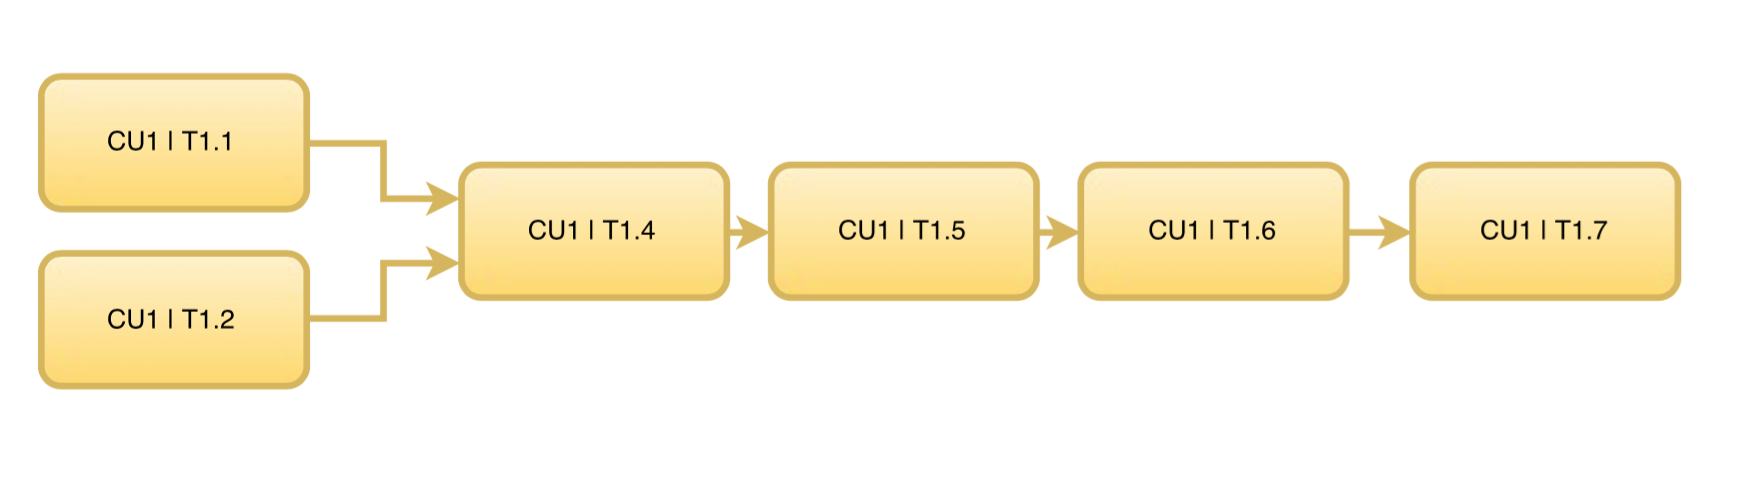
\includegraphics[width=15cm]{diagramas/diag-dependecias1.png}
    \caption{Diagrama de dependencias entre las tareas del CU nro 1.}
    \label{fig:diag-dependecias1}
  \end{figure}
\end{center}

\begin{center}
  \begin{figure}[h!]
    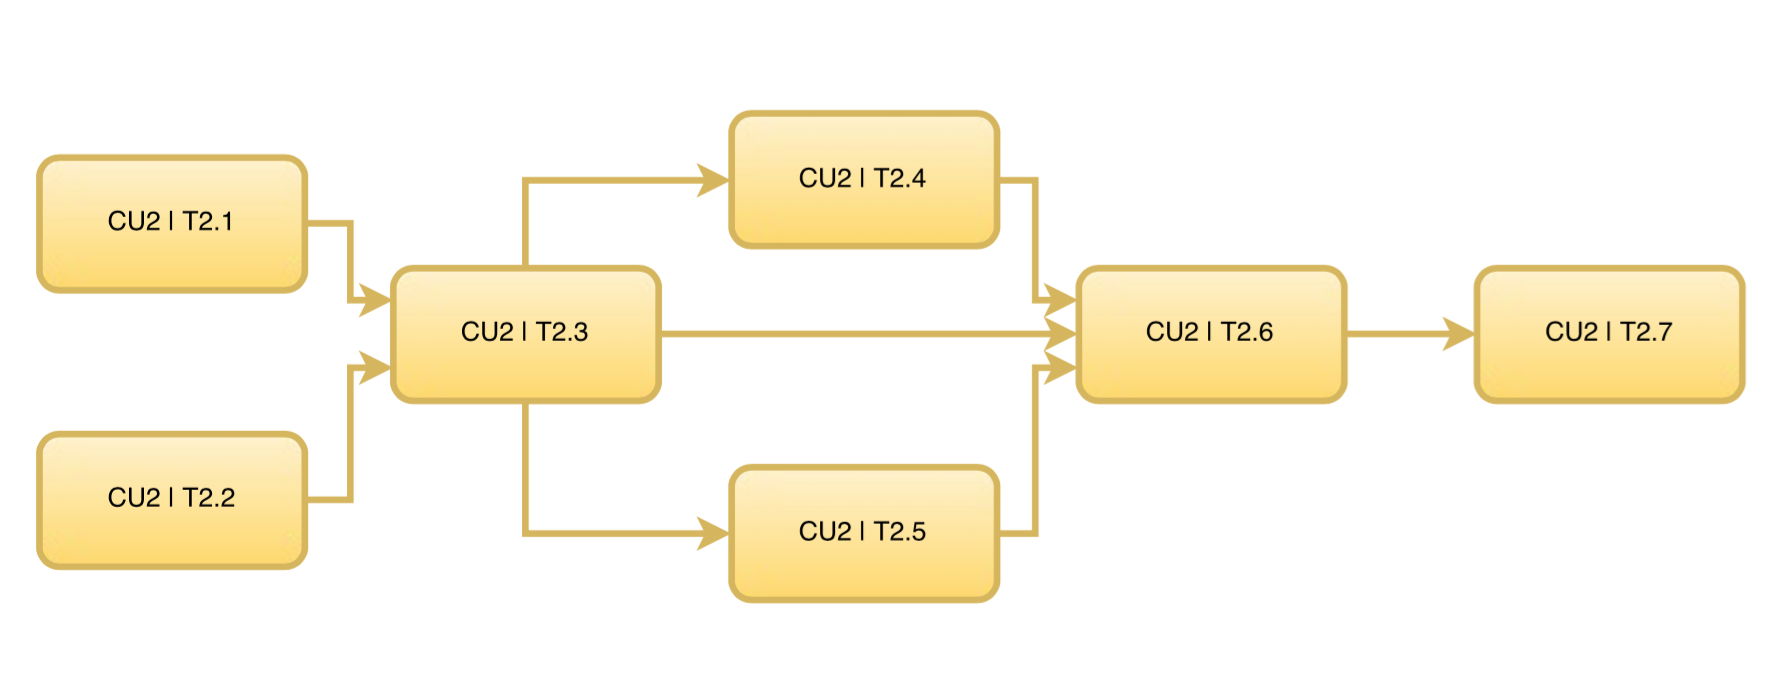
\includegraphics[width=15cm]{diagramas/diag-dependecias2.png}
    \caption{Diagrama de dependencias entre las tareas del CU nro 2.}
    \label{fig:diag-dependecias2}
  \end{figure}
\end{center}

\begin{center}
  \begin{figure}[h!]
    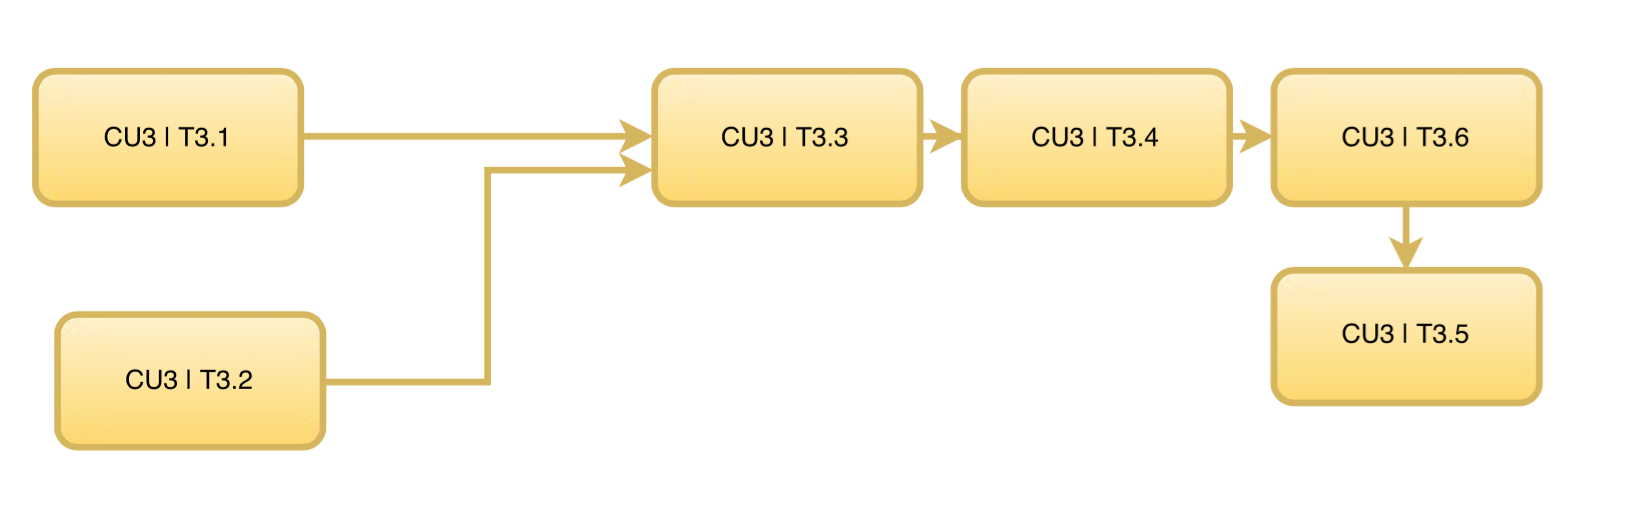
\includegraphics[width=15cm]{diagramas/diag-dependecias3.png}
    \caption{Diagrama de dependencias entre las tareas del CU nro 3.}
    \label{fig:diag-dependecias3}
  \end{figure}
\end{center}

\begin{center}
  \begin{figure}[h!]
    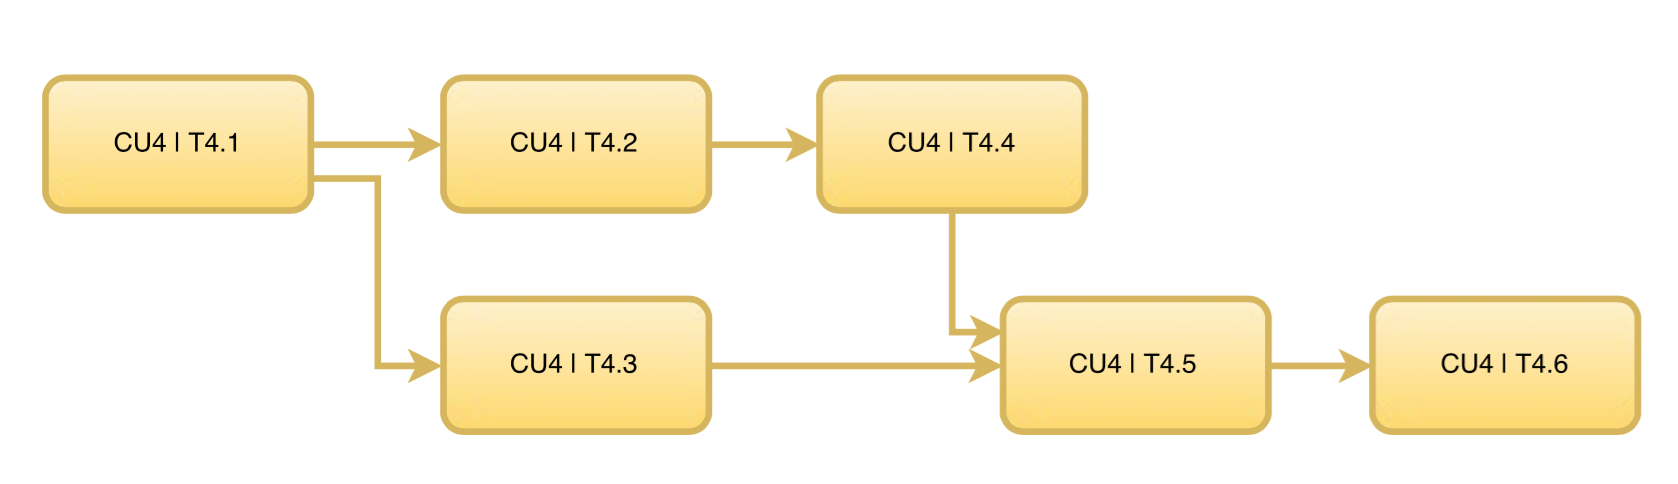
\includegraphics[width=15cm]{diagramas/diag-dependecias4.png}
    \caption{Diagrama de dependencias entre las tareas del CU nro 4.}
    \label{fig:diag-dependecias4}
  \end{figure}
\end{center}


\subsection{Detalle Primera iteración}

\begin{itemize}
  \item \textbf{Identificación:} E1
  \item \textbf{Tipo de iteración:} Elaboración
  \item \textbf{Cantidad total de horas:} 528
  \item \textbf{Tareas:}
\begin{enumerate}
  \item Definir organización de la base de código y sistema de versionado. (4h)
  \item Definir motor de base de datos a utilizar para datos de usuario. (8h)
  \item Desarrollar un servidor de integración continua y testing. (20h)
  \item Definir método de encriptación para contraseñas y datos sensibles. (10h)
  \item Definir conjunto de datos a persistir por cada usuario. (16h)
  \item Elegir lenguajes y plataformas para el desarrollo de cada subsistema. (10h)
  \item Establecer criterios de calidad y formato de código. (2h)
  \item Diseñar base de datos de usuarios. (10h)
  \item Desarrollar un servidor de deploy. (15h)
  \item Implementación de CU1 (40h)
  \item Testing de CU1 (30h)
  \item Investigar tecnologías web a utilizar para el cliente web. (16h)
  \item Investigar tecnologías a utilizar para los clientes móviles. (16h)
  \item Desarrollar stubs de las aplicaciones web y móviles. (8h)
  \item Integrar motor de gráficos 2D a la aplicación web. (18h)
  \item Integrar motor de gráficos 2D a la aplicación móvil. (18h)
  \item Implementación de una visualización de partido de prueba. (45h)
  \item Testing de CU2 (40h)
  \item Investigar plataforma para el servidor de transmisión. (10h)
  \item Definir la interfaz de comunicación con el servidor. (10h)
  \item Desarrollar stub del servidor. (8h)
  \item Implementar transmisión de datos de una simulación de prueba. (35h)
  \item Desarrollar cliente simple de prueba. (10h)
  \item Testing de CU3 (30h)
  \item Definir motor de base de datos a utilizar para datos de desafíos. (8h)
  \item Definir conjunto de datos a persistir por cada desafío. (10h)
  \item Investigar alternativas para la persistencia segura de datos del desafío. (10h)
  \item Diseñar base de datos de desafíos. (16h)
  \item Implementación de CU4 (30h)
  \item Testing de CU4 (25h)
\end{enumerate}
\end{itemize}

\subsection{Plan de Proyecto}

En el siguiente diagrama detallamos el plan de desarrollo del proyecto, con una planificación estimada del desarrollo de las tareas a realizar en la primera iteración. Para la distribución en tiempo de las mismas, se asignó el tiempo de cuatro desarrolladores con una dedicación de cuatro horas diarias al proyecto.


\begin{landscape}
\begin{center}
  \begin{figure}[h!]
    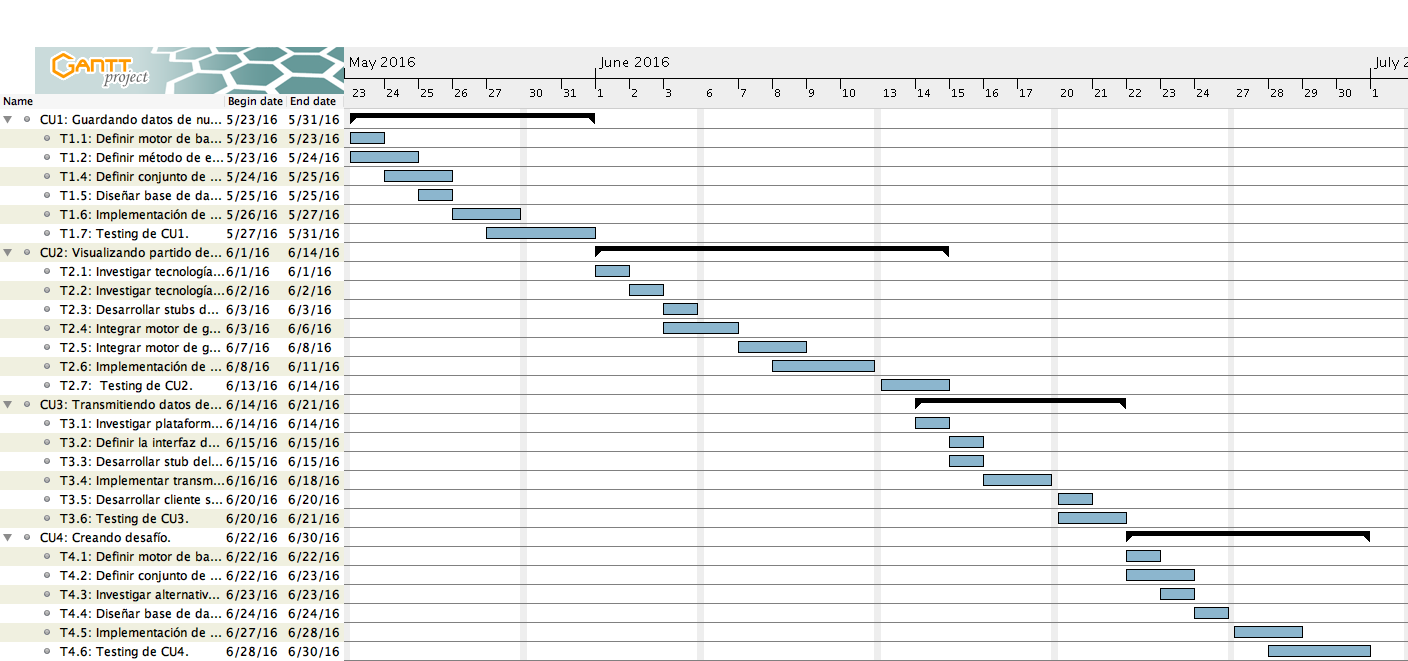
\includegraphics[width=25cm]{./diagramas/gantt.png}
    \caption{Diagrama de Gantt de la 1era iteración con la asignación de tiempo}
    \label{fig:gantt}
  \end{figure}
\end{center}
\end{landscape}
\newpage

%%%%%%%%%%%%%%%%%%%%%%%%%%%%%%%%%%%%%%%%%%%%%%%%%%%%%%%%%%%%%%%%%%%%%%%%%%%%%%%
%% Análisis de riesgo                                                        %%
%%%%%%%%%%%%%%%%%%%%%%%%%%%%%%%%%%%%%%%%%%%%%%%%%%%%%%%%%%%%%%%%%%%%%%%%%%%%%%%

\section{Análisis de riesgos}
\label{riesgos:r1}
\riesgo{1}
    { Los motores gráficos 2D y 3D son desarrollados por terceros. Si alguna de las dos compañías deja de funcionar, perdemos soporte para el correspondiente motor gráfico e incrementa fuertemente el costo y tiempo de desarrollo para realizar mejoras o agregar funcionalidad en el mismo. }
    {Baja} % Probabilidad
    {Alto} % Impacto
    {Media} % Exposición
    {Establecer una capa de abtracción encima de los motores gráficos para que los mismos sean reemplazables sin que sea necesario modificar los demás sistemas.} % Mitigación
    {Licitar el motor gráfico que ha perdido soporte entre nuevas empresas.} % Plan de contingencia

\riesgo{2}
    {Actualmente, los usuarios tienen múltiples modos para visualizar un partido: simulación 2D o 3D a partir del feed de la simulación, streaming de partidos reales y streaming de un render de la simulación realizado del lado del servidor. Si un usuario tiene un dispositivo sin las prestaciones necesarias para realizar una simulación de forma nativa, cada vez que tenga mala conectividad tampoco será capaz de visualizar streamings y no podrá obtener información sobre los partidos de ninguna manera. }
    {Media} % Probabilidad
    {Medio} % Impacto
    {Media} % Exposición
    {Desarrollar un feed de información acerca del partido en ejecución que sea apto para clientes con bajos recursos de hardware y mala conectividad.}
    {Proponer al usuario afectado la visualización del feed del partido basado en texto.}

\riesgo{3}
    {El sistema en su conjunto procesa varios conjuntos de datos altamente sensibles que refieren a la identidad de sus usuarios, a sus medios de pago, y la realización de las simulaciones que determinan los desafíos para bajo apuestas o con premios, así como los resultados de los mismos. Si alguno de estos sistemas es comprometido, la integridad personal o económica de los usuarios o del sistema mismo pueden sufrir consecuencias irreversibles. }
    {Media} % Probabilidad
    {Alto} % Impacto
    {Media} % Exposición
    {Investigar fuertemente las mejores prácticas en seguridad para el desarrollo de los sistemas que procesan información sensible.}
    {Suspensión inmediata de actividades en la platafoma con posibles resultados irreversibles (pagos, entrega de premios) e investigación sobre el siniestro cooperando con las autoridades.}

\newpage


\section{Atributos de calidad}


\subsection{Disponibilidad}

\begin{center}
  \begin{tabular}{| l | p{10cm} | }
    \hline
  \textbf{Descripción} & Los partidos deben servirse con excelente calidad y sin cortes a pesar de que servidores de la empresa proveedora se pueden caer sin previo aviso.\\  \hline
  \textbf{Fuente} & Servidor del proveedor\\  \hline
  \textbf{Estímulo} & Se cae, por lo tanto deja de enviar datos.\\  \hline
  \textbf{Entorno} & Normal\\  \hline
  \textbf{Artefacto} & Sistema\\  \hline
  \textbf{Respuesta} & Se identifica la ca'ida del server por timeout y se inicia una nueva comunicaci'on con otro server.\\  \hline
  \textbf{Medición} & El tamano del buffer de streaming es suficiente para que s'olo se perciba la ca'ida 0,001 seg/hora dada que el uptime de los proveedores del servidor es de 95\%.\\  \hline
  \end{tabular}
\end{center} 

%% \begin{center}
%%   \begin{tabular}{| l | p{10cm} | }
%%     \hline
%%   \textbf{Descripción} & Los servidores de streaming de cada region deben ser acordes a la calidad de video usualmente transmitida a los usuarios de dicha region.\\  \hline
%%   \textbf{Fuente} & UNA FUENTE\\  \hline
%%   \textbf{Estímulo} & UN ESTIMULO.\\  \hline
%%   \textbf{Entorno} & UN ENTORNO\\  \hline
%%   \textbf{Artefacto} & UN ARTEFACTO\\  \hline
%%   \textbf{Respuesta} & UNA RESPUESTA\\  \hline
%%   \textbf{Medición} & UNA MEDICION\\  \hline
%%   \end{tabular}
%% \end{center} 

\begin{center}
  \begin{tabular}{| l | p{10cm} | }
    \hline
  \textbf{Descripción} & El sistema debe evitar que los servidores superen su l'imite de clientes y se caigan.\\  \hline
  \textbf{Fuente} & Usuario\\  \hline
  \textbf{Estímulo} & Se hace un pedido.\\  \hline
  \textbf{Entorno} & Sistema con servidor saturado\\  \hline
  \textbf{Artefacto} & Sistema\\  \hline
  \textbf{Respuesta} & Se selecciona un servidor que no est'a saturado y se direcciona al cliente a 'el.\\  \hline
  \textbf{Medición} & El 0.01\% de veces un servidor se satura y se direcciona un cliente a 'el antes de que la notificaci'on de que est'a saturado llegue al router.\\  \hline
  \end{tabular}
\end{center} 

\begin{center}
  \begin{tabular}{| l | p{10cm} | }
    \hline
  \textbf{Descripción} & Desea que haya un esfuerzo por respetar a los países en los que su legislación no permite que directamente se ingrese al sitio.\\  \hline
  \textbf{Fuente} & UNA FUENTE\\  \hline
  \textbf{Estímulo} & UN ESTIMULO.\\  \hline
  \textbf{Entorno} & UN ENTORNO\\  \hline
  \textbf{Artefacto} & UN ARTEFACTO\\  \hline
  \textbf{Respuesta} & UNA RESPUESTA\\  \hline
  \textbf{Medición} & UNA MEDICION\\  \hline
  \end{tabular}
\end{center} 


\begin{center}
  \begin{tabular}{| l | p{10cm} | }
    \hline
  \textbf{Descripción} & Se requiere que sea fácil desactivar una cuenta por un tiempo, para ayudar a los adictos en recuperación.\\  \hline
  \textbf{Fuente} & Usuario adicto\\  \hline
  \textbf{Estímulo} & Un usuario adicto intenta conectarce.\\  \hline
  \textbf{Entorno} & Normal\\  \hline
  \textbf{Artefacto} & Sistema\\  \hline
  \textbf{Respuesta} & Se bloquea el acceso al sistema.\\  \hline
  \textbf{Medición} & El 99,99\% de los casos que un usuario adicto intenta conectarse desde una cuenta desactivada el acceso al sistema es bloqueado.\\  \hline
  \end{tabular}
\end{center} 





\subsection{Modificabilidad}

\begin{center}
  \begin{tabular}{| l | p{10cm} | }
    \hline
  \textbf{Descripción} & El simulador debe poder extenderse para soportar reglamentaciones nuevas ya que se espera poder incluir pa'ises adicionales.\\  \hline
  \textbf{Fuente} & UNA FUENTE\\  \hline
  \textbf{Estímulo} & UN ESTIMULO.\\  \hline
  \textbf{Entorno} & UN ENTORNO\\  \hline
  \textbf{Artefacto} & UN ARTEFACTO\\  \hline
  \textbf{Respuesta} & UNA RESPUESTA\\  \hline
  \textbf{Medición} & UNA MEDICION\\  \hline
  \end{tabular}
\end{center} 

\begin{center}
  \begin{tabular}{| l | p{10cm} | }
    \hline
  \textbf{Descripción} & El sistema debe correr en la mayor cantidad de plataformas posible. El sistema debe poder extenderse f'acilmente para incluir nueva.\\  \hline
  \textbf{Fuente} & UNA FUENTE\\  \hline
  \textbf{Estímulo} & UN ESTIMULO.\\  \hline
  \textbf{Entorno} & UN ENTORNO\\  \hline
  \textbf{Artefacto} & UN ARTEFACTO\\  \hline
  \textbf{Respuesta} & UNA RESPUESTA\\  \hline
  \textbf{Medición} & UNA MEDICION\\  \hline
  \end{tabular}
\end{center} 

\begin{center}
  \begin{tabular}{| l | p{10cm} | }
    \hline
  \textbf{Descripción} & Se deben poder agregar nuevos criterios para hacer data mining f'acilmente.\\  \hline
  \textbf{Fuente} & UNA FUENTE\\  \hline
  \textbf{Estímulo} & UN ESTIMULO.\\  \hline
  \textbf{Entorno} & UN ENTORNO\\  \hline
  \textbf{Artefacto} & UN ARTEFACTO\\  \hline
  \textbf{Respuesta} & UNA RESPUESTA\\  \hline
  \textbf{Medición} & UNA MEDICION\\  \hline
  \end{tabular}
\end{center} 
\begin{center}
  \begin{tabular}{| l | p{10cm} | }
    \hline
  \textbf{Descripción} & Deben poder crearse nuevos desaf'ios en base a los datos minados.\\  \hline
  \textbf{Fuente} & UNA FUENTE\\  \hline
  \textbf{Estímulo} & UN ESTIMULO.\\  \hline
  \textbf{Entorno} & UN ENTORNO\\  \hline
  \textbf{Artefacto} & UN ARTEFACTO\\  \hline
  \textbf{Respuesta} & UNA RESPUESTA\\  \hline
  \textbf{Medición} & UNA MEDICION\\  \hline
  \end{tabular}
\end{center} 

\begin{center}
  \begin{tabular}{| l | p{10cm} | }
    \hline
  \textbf{Descripción} & Se quiere poder controlar las publicidades en las simulaciones y el sitio en general en base a el tipo de audencia.\\  \hline
  \textbf{Fuente} & UNA FUENTE\\  \hline
  \textbf{Estímulo} & UN ESTIMULO.\\  \hline
  \textbf{Entorno} & UN ENTORNO\\  \hline
  \textbf{Artefacto} & UN ARTEFACTO\\  \hline
  \textbf{Respuesta} & UNA RESPUESTA\\  \hline
  \textbf{Medición} & UNA MEDICION\\  \hline
  \end{tabular}
\end{center} 

\begin{center}
  \begin{tabular}{| l | p{10cm} | }
    \hline
  \textbf{Descripción} & Deben poder adaptarse los mecanismos de streaming segun la region. \\  \hline
  \textbf{Fuente} & UNA FUENTE\\  \hline
  \textbf{Estímulo} & UN ESTIMULO.\\  \hline
  \textbf{Entorno} & UN ENTORNO\\  \hline
  \textbf{Artefacto} & UN ARTEFACTO\\  \hline
  \textbf{Respuesta} & UNA RESPUESTA\\  \hline
  \textbf{Medición} & UNA MEDICION\\  \hline
  \end{tabular}
\end{center} 

\begin{center}
  \begin{tabular}{| l | p{10cm} | }
    \hline
  \textbf{Descripción} & Poder agreger, borrar, modificar ads y publicidades que se van a ver durante las transmiciones de los partidos.\\  \hline
  \textbf{Fuente} & UNA FUENTE\\  \hline
  \textbf{Estímulo} & UN ESTIMULO.\\  \hline
  \textbf{Entorno} & UN ENTORNO\\  \hline
  \textbf{Artefacto} & UN ARTEFACTO\\  \hline
  \textbf{Respuesta} & UNA RESPUESTA\\  \hline
  \textbf{Medición} & UNA MEDICION\\  \hline
  \end{tabular}
\end{center} 

\begin{center}
  \begin{tabular}{| l | p{10cm} | }
    \hline
  \textbf{Descripción} & Toda la simulación pueda irse mejorando poco a poco hasta que represente lo mejor posible la realidad sin que sea un dolor de cabeza introducir cambios\\  \hline
  \textbf{Fuente} & UNA FUENTE\\  \hline
  \textbf{Estímulo} & UN ESTIMULO.\\  \hline
  \textbf{Entorno} & UN ENTORNO\\  \hline
  \textbf{Artefacto} & UN ARTEFACTO\\  \hline
  \textbf{Respuesta} & UNA RESPUESTA\\  \hline
  \textbf{Medición} & UNA MEDICION\\  \hline
  \end{tabular}
\end{center} 

\begin{center}
  \begin{tabular}{| l | p{10cm} | }
    \hline
  \textbf{Descripción} & Tiene que ser escalable a partir de “cosas chicas” o va a haber problemas. \\  \hline
  \textbf{Fuente} & UNA FUENTE\\  \hline
  \textbf{Estímulo} & UN ESTIMULO.\\  \hline
  \textbf{Entorno} & UN ENTORNO\\  \hline
  \textbf{Artefacto} & UN ARTEFACTO\\  \hline
  \textbf{Respuesta} & UNA RESPUESTA\\  \hline
  \textbf{Medición} & UNA MEDICION\\  \hline
  \end{tabular}
\end{center} 




\subsection{Usabilidad}

\begin{center}
  \begin{tabular}{| l | p{10cm} | }
    \hline
  \textbf{Descripción} & Que los datos queden resguardados y sólo haya que actualizarlos esporádicamente\\  \hline
  \textbf{Fuente} & UNA FUENTE\\  \hline
  \textbf{Estímulo} & UN ESTIMULO.\\  \hline
  \textbf{Entorno} & UN ENTORNO\\  \hline
  \textbf{Artefacto} & UN ARTEFACTO\\  \hline
  \textbf{Respuesta} & UNA RESPUESTA\\  \hline
  \textbf{Medición} & UNA MEDICION\\  \hline
  \end{tabular}
\end{center} 

\begin{center}
  \begin{tabular}{| l | p{10cm} | }
    \hline
  \textbf{Descripción} & Le interesa que la interfaz gráfica de usuarios tenga la calidad de un “juego”, sobre toda al momento de ver a los jugadores, las jugadas de los técnicos, colocar el nombre y logo del equipo del participante, etc… con animaciones y efectos especiales con aceleración gráfica (blurs, iluminación dinámica, depth of field, etc). \\  \hline
  \textbf{Fuente} & UNA FUENTE\\  \hline
  \textbf{Estímulo} & UN ESTIMULO.\\  \hline
  \textbf{Entorno} & UN ENTORNO\\  \hline
  \textbf{Artefacto} & UN ARTEFACTO\\  \hline
  \textbf{Respuesta} & UNA RESPUESTA\\  \hline
  \textbf{Medición} & UNA MEDICION\\  \hline
  \end{tabular}
\end{center} 

\begin{center}
  \begin{tabular}{| l | p{10cm} | }
    \hline
  \textbf{Descripción} & Quiere poder definir los ads y publicidades que se van a ver durante las transmisiones de los partidos que ellos tienen derechos a través de una interfaz gráfica que permite elegirlos (ABM) para diferentes audiencias (tipos de usuarios)\\  \hline
  \textbf{Fuente} & UNA FUENTE\\  \hline
  \textbf{Estímulo} & UN ESTIMULO.\\  \hline
  \textbf{Entorno} & UN ENTORNO\\  \hline
  \textbf{Artefacto} & UN ARTEFACTO\\  \hline
  \textbf{Respuesta} & UNA RESPUESTA\\  \hline
  \textbf{Medición} & UNA MEDICION\\  \hline
  \end{tabular}
\end{center} 

\begin{center}
  \begin{tabular}{| l | p{10cm} | }
    \hline
  \textbf{Descripción} & Quiere poder que él y sus administradores de confianza puedan ver un dashboard en tiempo real del estado de cuenta del sitio de cada una de las regiones y niveles (incluye locales, continentales, global, etc…) y de cualquier grupo de participantes. 
\\  \hline
  \textbf{Fuente} & UNA FUENTE\\  \hline
  \textbf{Estímulo} & UN ESTIMULO.\\  \hline
  \textbf{Entorno} & UN ENTORNO\\  \hline
  \textbf{Artefacto} & UN ARTEFACTO\\  \hline
  \textbf{Respuesta} & UNA RESPUESTA\\  \hline
  \textbf{Medición} & UNA MEDICION\\  \hline
  \end{tabular}
\end{center} 

















\subsection{Performance}



\begin{center}
  \begin{tabular}{| l | p{10cm} | }
    \hline
  \textbf{Descripción} & Acepta sin embargo las calidades diferentes en base a un bitrate variable y el bandwidth de conexión de cada usuario.\\  \hline
  \textbf{Fuente} & UNA FUENTE\\  \hline
  \textbf{Estímulo} & UN ESTIMULO.\\  \hline
  \textbf{Entorno} & UN ENTORNO\\  \hline
  \textbf{Artefacto} & UN ARTEFACTO\\  \hline
  \textbf{Respuesta} & UNA RESPUESTA\\  \hline
  \textbf{Medición} & UNA MEDICION\\  \hline
  \end{tabular}
\end{center} 



\begin{center}
  \begin{tabular}{| l | p{10cm} | }
    \hline
  \textbf{Descripción} & mientras sea posible se use el engine 3d de mayor calidad al 2d.\\  \hline
  \textbf{Fuente} & UNA FUENTE\\  \hline
  \textbf{Estímulo} & UN ESTIMULO.\\  \hline
  \textbf{Entorno} & UN ENTORNO\\  \hline
  \textbf{Artefacto} & UN ARTEFACTO\\  \hline
  \textbf{Respuesta} & UNA RESPUESTA\\  \hline
  \textbf{Medición} & UNA MEDICION\\  \hline
  \end{tabular}
\end{center} 



\begin{center}
  \begin{tabular}{| l | p{10cm} | }
    \hline
  \textbf{Descripción} & Los eventos globales deben funcionar correctamente.\\  \hline
  \textbf{Fuente} & UNA FUENTE\\  \hline
  \textbf{Estímulo} & UN ESTIMULO.\\  \hline
  \textbf{Entorno} & UN ENTORNO\\  \hline
  \textbf{Artefacto} & UN ARTEFACTO\\  \hline
  \textbf{Respuesta} & UNA RESPUESTA\\  \hline
  \textbf{Medición} & UNA MEDICION\\  \hline
  \end{tabular}
\end{center} 


\subsection{Seguridad}

\begin{center}
  \begin{tabular}{| l | p{10cm} | }
    \hline
  \textbf{Descripción} & Todo lo respectivo al manejo de dinero sea seguro.\\  \hline
  \textbf{Fuente} & UNA FUENTE\\  \hline
  \textbf{Estímulo} & UN ESTIMULO.\\  \hline
  \textbf{Entorno} & UN ENTORNO\\  \hline
  \textbf{Artefacto} & UN ARTEFACTO\\  \hline
  \textbf{Respuesta} & UNA RESPUESTA\\  \hline
  \textbf{Medición} & UNA MEDICION\\  \hline
  \end{tabular}
\end{center} 

\begin{center}
  \begin{tabular}{| l | p{10cm} | }
    \hline
  \textbf{Descripción} & Todo lo respectivo al manejo de dinero sea transparente.\\  \hline
  \textbf{Fuente} & UNA FUENTE\\  \hline
  \textbf{Estímulo} & UN ESTIMULO.\\  \hline
  \textbf{Entorno} & UN ENTORNO\\  \hline
  \textbf{Artefacto} & UN ARTEFACTO\\  \hline
  \textbf{Respuesta} & UNA RESPUESTA\\  \hline
  \textbf{Medición} & UNA MEDICION\\  \hline
  \end{tabular}
\end{center} 

\begin{center}
  \begin{tabular}{| l | p{10cm} | }
    \hline
  \textbf{Descripción} & Todo lo respectivo al manejo de dinero sea rapido.\\  \hline
  \textbf{Fuente} & UNA FUENTE\\  \hline
  \textbf{Estímulo} & UN ESTIMULO.\\  \hline
  \textbf{Entorno} & UN ENTORNO\\  \hline
  \textbf{Artefacto} & UN ARTEFACTO\\  \hline
  \textbf{Respuesta} & UNA RESPUESTA\\  \hline
  \textbf{Medición} & UNA MEDICION\\  \hline
  \end{tabular}
\end{center} 

\begin{center}
  \begin{tabular}{| l | p{10cm} | }
    \hline
  \textbf{Descripción} & Los datos de usuarios no se deben poder robar, tienen que tener confidencialidad y autenticidad. (datos de tarjetas, etc). \\  \hline
  \textbf{Fuente} & UNA FUENTE\\  \hline
  \textbf{Estímulo} & UN ESTIMULO.\\  \hline
  \textbf{Entorno} & UN ENTORNO\\  \hline
  \textbf{Artefacto} & UN ARTEFACTO\\  \hline
  \textbf{Respuesta} & UNA RESPUESTA\\  \hline
  \textbf{Medición} & UNA MEDICION\\  \hline
  \end{tabular}
\end{center} 

\begin{center}
  \begin{tabular}{| l | p{10cm} | }
    \hline
  \textbf{Descripción} & Se teme por el resultado de los desafiıos, el pago/cobro a los participantes y la coherencia con los datos provenientes de las empresas que relevan los resultados de los partidos. \\  \hline
  \textbf{Fuente} & UNA FUENTE\\  \hline
  \textbf{Estímulo} & UN ESTIMULO.\\  \hline
  \textbf{Entorno} & UN ENTORNO\\  \hline
  \textbf{Artefacto} & UN ARTEFACTO\\  \hline
  \textbf{Respuesta} & UNA RESPUESTA\\  \hline
  \textbf{Medición} & UNA MEDICION\\  \hline
  \end{tabular}
\end{center} 

\begin{center}
  \begin{tabular}{| l | p{10cm} | }
    \hline
  \textbf{Descripción} & Teme por la transparencia del funcionamiento de las simulaciones. Quiere que los módulos de las simulaciones puedan ser inspeccionadas fácilmente por entidades de control para verificar que su funcionamiento no es fraudulento. Le gustaría poder reproducir las mismas en sistemas testigo para verificar resultados.\\  \hline
  \textbf{Fuente} & UNA FUENTE\\  \hline
  \textbf{Estímulo} & UN ESTIMULO.\\  \hline
  \textbf{Entorno} & UN ENTORNO\\  \hline
  \textbf{Artefacto} & UN ARTEFACTO\\  \hline
  \textbf{Respuesta} & UNA RESPUESTA\\  \hline
  \textbf{Medición} & UNA MEDICION\\  \hline
  \end{tabular}
\end{center} 

\begin{center}
  \begin{tabular}{| l | p{10cm} | }
    \hline
  \textbf{Descripción} & Quiere que se “loguee” cada movimiento de dinero, sin importar su monto, pues los gobiernos no van a permitir ningun tipo de evasión impositiva por las ganancias de la empresa en su región. \\  \hline
  \textbf{Fuente} & UNA FUENTE\\  \hline
  \textbf{Estímulo} & UN ESTIMULO.\\  \hline
  \textbf{Entorno} & UN ENTORNO\\  \hline
  \textbf{Artefacto} & UN ARTEFACTO\\  \hline
  \textbf{Respuesta} & UNA RESPUESTA\\  \hline
  \textbf{Medición} & UNA MEDICION\\  \hline
  \end{tabular}
\end{center} 


\section{Arquitectura}
\subsection{Conectores propios}
\subsubsection{Notaci'on}

\begin{itemize}
\item Pipe 
\includegraphics[height=0.6cm]{diagramas/NPIPE} 
\item HC (Holy Connector) 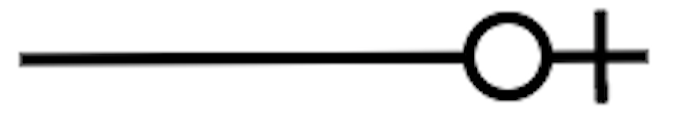
\includegraphics[height=0.5cm]{diagramas/NHC} 
\item AHC (Asynchronous Holy Connector) 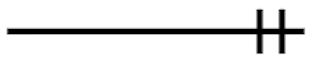
\includegraphics[height=0.5cm]{diagramas/NHCCA}
\item HVC (Holy Video Connector) 
\includegraphics[height=0.5cm]{diagramas/NHVC} 
\item HDC (Holy Data Connector) 
\includegraphics[height=0.5cm]{diagramas/NHDC} 

\end{itemize}

\subsubsection{HC (Holy Connector)}

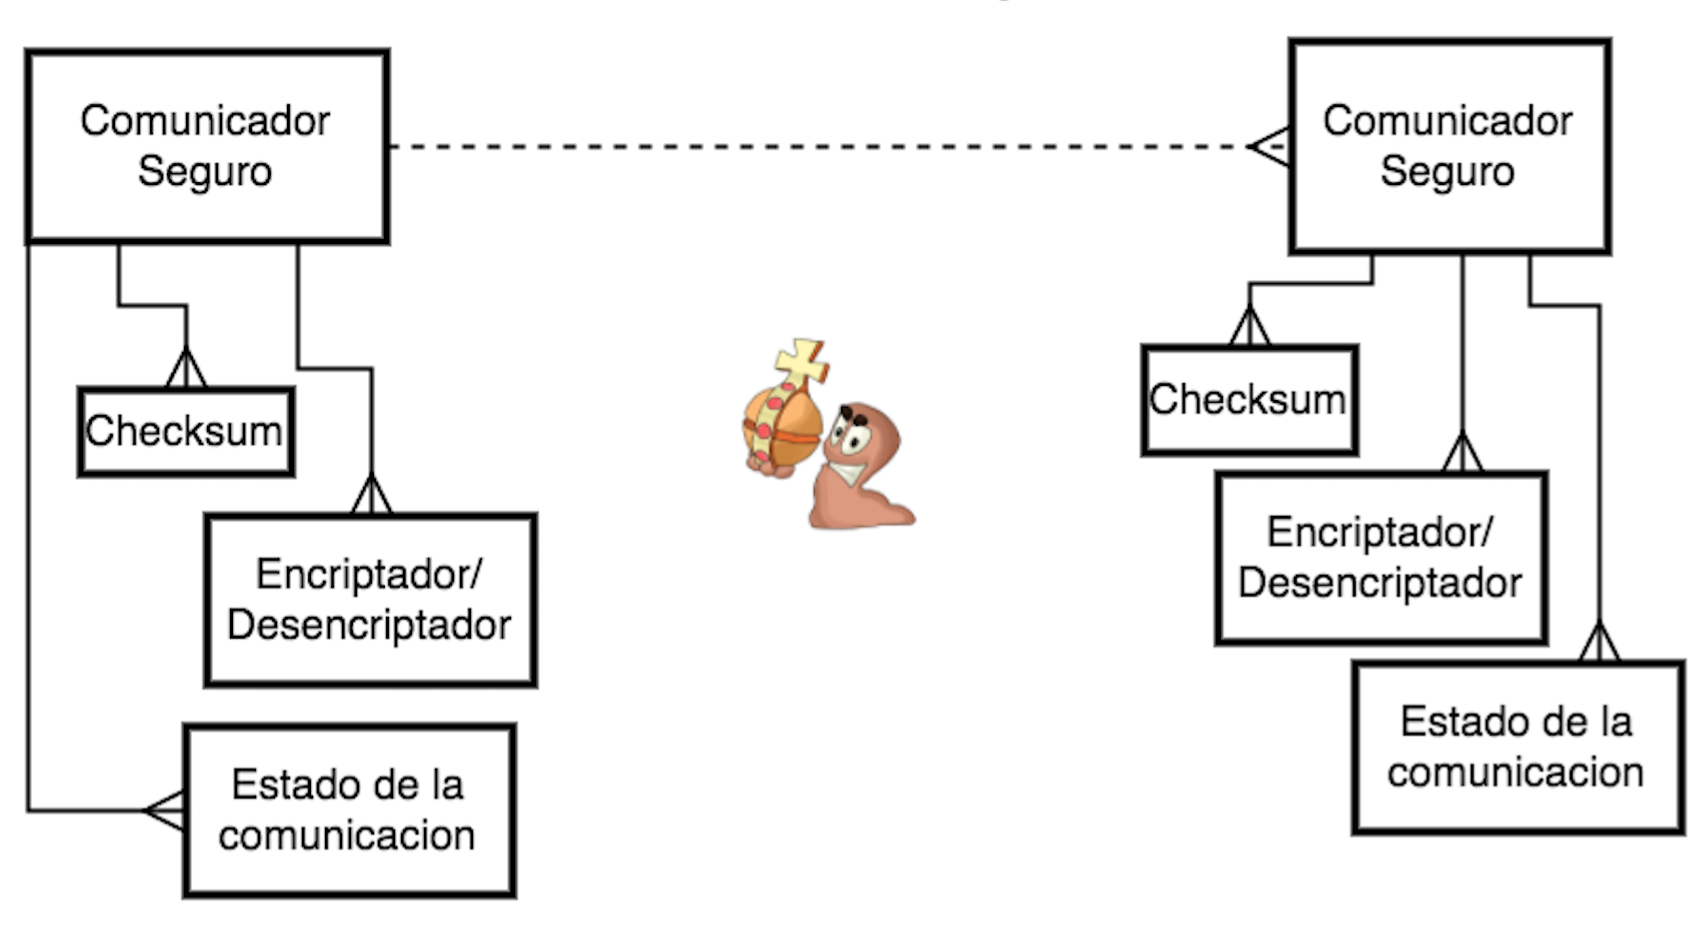
\includegraphics[height=9cm]{diagramas/HC} 

Este conector provee:

\begin{itemize}
	\item \textbf{Seguridad.} Mediante un componente de encriptaci'on y desencriptaci'on de los datos enviados.
	\item \textbf{Integridad.} Mediante un componente de checksum.
	\item \textbf{Confiabilidad de la conexi'on.} Mediante un componente que mantiene el estado de la conexi'on. Por ejemplo, este componente podr'ia implementar el protocolo TCP.
\end{itemize}

Observemos que entre los extremos utilizamos un conector tipo client-server que, asumimos, que se extiende sobre un medio inseguro. Por lo tanto, podemos pensar al Holy Connector como un cliente-server seguro, sobre un medio inseguro.

\subsubsection{AHC (Asynchronous Holy Connector)}

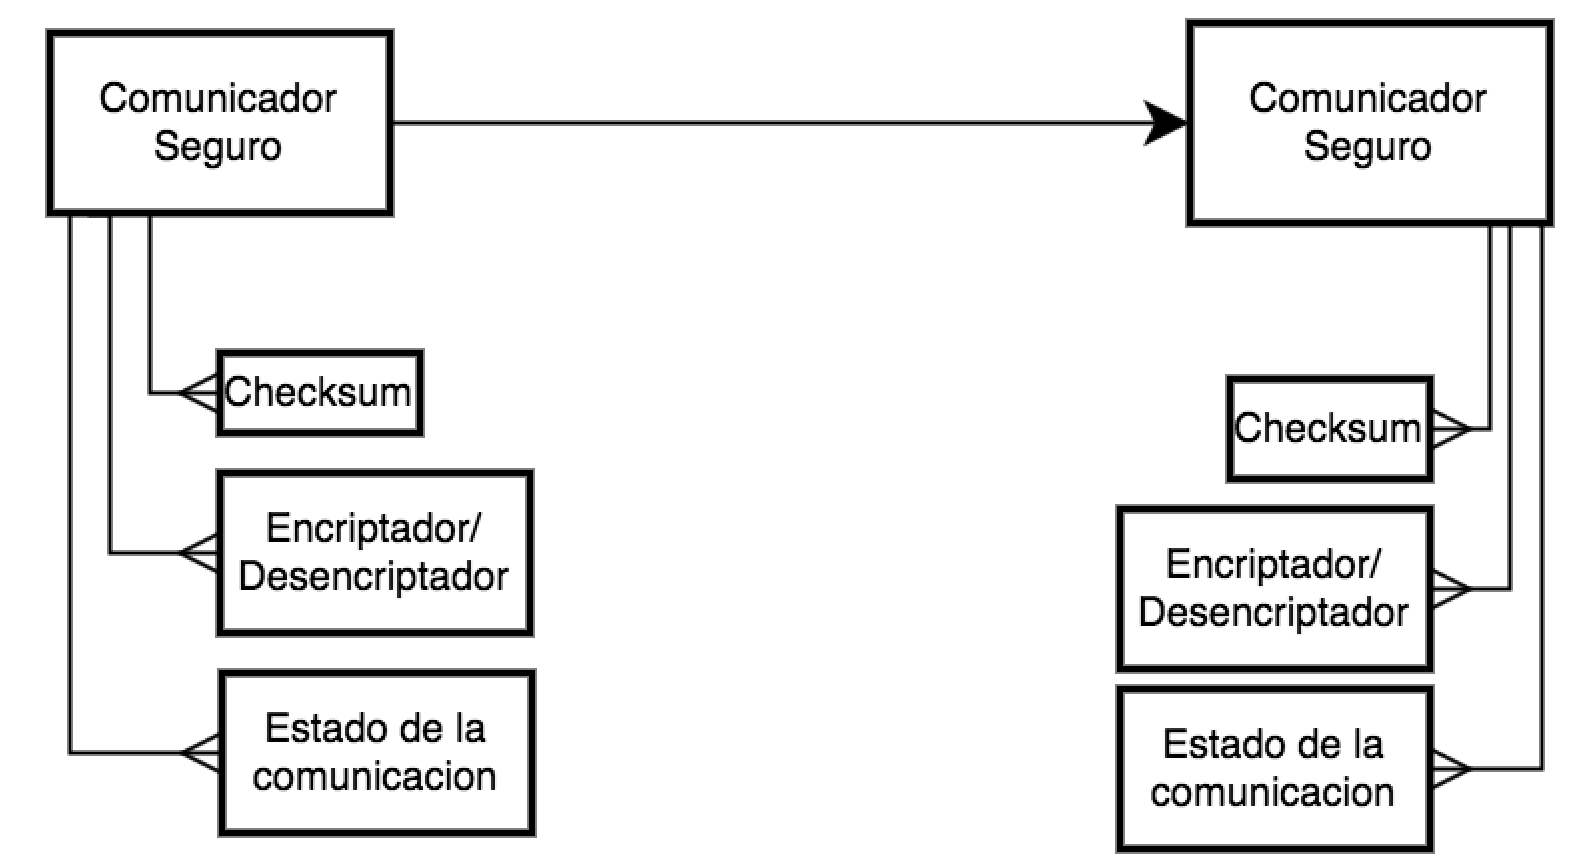
\includegraphics[height=9cm]{diagramas/HCCA} 

Id'entico al Holy Connector, con la diferencia de que en lugar de usar un client-server como conector intermedio, utilizamos un conector de call asincr'onico.

\subsubsection{HVC (Holy Video Connector)}

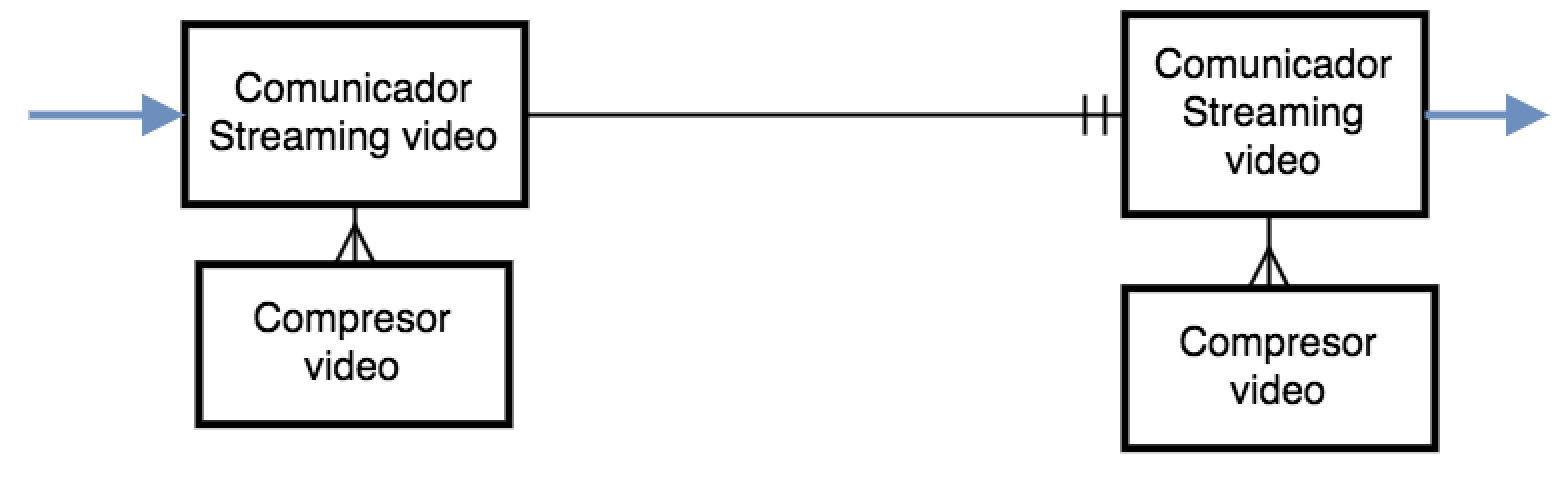
\includegraphics[height=5cm]{diagramas/HVC} 

Contamos en ambos extremos con comunicadores de streaming, que se comunican mediante un Holy Connector. Adicionalmente tenemos, en ambos extremos, compresores adecuados, para que la tasa de cantidad de informaci'on transmitida sea m'as alta.

En ambos extremos tenemos, adem'as, pipes como conectores de entrada y salida. Este buffering permite el env'io y recepci'on de datos flu'ida (evita los tipicos mensajes ``\textbf{buffering...}'').


\subsubsection{HDC (Holy Data Connector)}

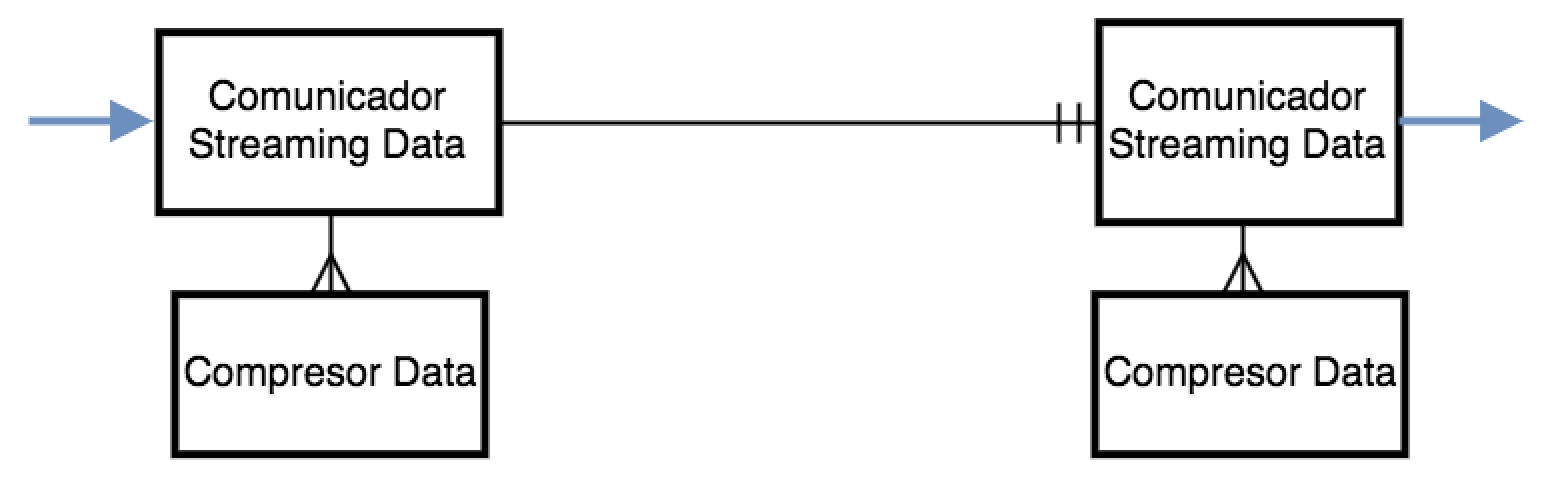
\includegraphics[height=5cm]{diagramas/HDC} 

An'alogo al HVC, pero con compresores adecuados para texto en lugar de video. 

\subsection{Diagrama}

\subsubsection{Descripci'on general}

Para describir la arquitectura, optamos por explicar c'omo se satisface cada una de los requerimientos indicados en el enunciado.

\textit{Lo primero que se pretende es que abarque varios de los deportes colectivos más populares del planeta. Además del ya citado básquet, deberá incorporar a las ligas de fútbol, hockey, rugby, béisbol y fútbol americano que se determine tengan mayor número de seguidores (ej. el fútbol español o la NFL estadounidense), y que se consigan empresas que provean datos en tiempo real de la evolución del partido (tanto del desempeño de los jugadores como del partido en general). Esto último es importante porque además de la simulación de los mismos, ahora también se quiere incorporar un modo de liga de fantasía tradicional.}

Para agregar deportes, lo 'unico que se debe hacer es contratar nuevos servicios de transmisi'on de partidos, agregar nuevos par'ametros del juego (i. e. agregar datos al repositorio de \textit{puntajes por acci'on}), y agregar funcionalidad al \textit{administrador de desaf'ios} para que se puedan crear desaf'ios de 'este nuevo deporte.

Los datos de la evoluci'on del partido provienen de los mismos servicios que nos transmiten partidos reales. Tanto los datos de un partido, como la transmisi'on del mismo nos son transmitidos en conjunto. Ver componente \textit{Servicio de transmisi'on de partido real}.

\textit{En este nuevo modo los ganadores de los desafíos ya no se deciden a través de la simulación directa de los partidos, sino del desempeño de los jugadores en partidos reales en las ligas en cuestión. Por ej. usando el caso del básquet, se podría otorgar 1 punto por cada punto que haga ese jugador en el partido, 1.5 puntos por cada asistencia, 2 por cada bloqueo o robo, -1 por cada pérdida de balón, etc... El equipo que tenga mayor suma, gana el desafío.}

El puntaje que se asigna a cada acci'on de cada deporte es un par'ametro que se encuentra en el repositorio \textit{puntajes por acci'on}.

\textit{Con respecto a los desafíos, ahora pueden incluir un gran número de partidos, no sólo uno. En el caso de este nuevo modo ``liga fantasía tradicional'', podrían incluirse todos los partidos de una fecha determinada de una liga, o un salteado de un conjunto de fechas cualesquiera, o incluso la liga o torneo completo.}

Los desaf'ios son creados por un cliente (un jugador) desde la pantalla de lista de desaf'ios, mediante el m'odulo \textit{creador de desaf'ios}. 'Este le env'ia un pedido al 



\subsubsection{Arquitectura de datacenters}

Nuestro sistema tiene una arquitectura distribuida, basada en datacenters. Un datacenter contiene una gran cantidad de servidores que proveen el servicio de juego. Dentro de un datacenter, los servidores se dividen en conjuntos, y cada conjunto provee servicio a una regi'on distinta. En otras palabras, un datacenter puede proveer servicio a distintas regiones por medio de cierto conjunto de servidores.

Todas las peticiones ingresantes en un datacenter son recibidas y procesadas por una m'aquina de tipo \textit{router}. Un router redirige la petici'on a alg'un servidor de la regi'on correspondiente. Los routers pueden rutear al conjunto de servidores de cualquiera de las regiones servidas en el datacenter. Por ejemplo, podr'ia haber un datacenter en Argentina, que provea el servicio para Argentina, Brasil y Uruguay; en este caso, los routers del datacenter procesan peticiones de las tres regiones.

El siguiente diagrama muestra lo descripto.

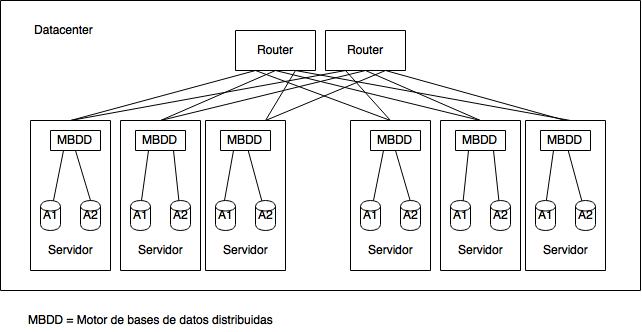
\includegraphics[width=15cm]{diagramas/datacenter.png}

\noindent
El datacenter de la figura tiene dos routers, que procesan pedidos para dos regiones. Cada regi'on se compone de tres servidores. Notar que una de las regiones contiene dos tipos de repositorios, A1 y A2. Estos repositorios aparecen en todos los servidores de la regi'on, debido a que los datos est'an distribuidos sobre todos estos servidores. An'alogamente, los servidores de la otra regi'on, tienen repositorios B1 y B2, distribuidos.

Cada servidor tiene un componente, denominado \textit{agente}. Un agente es la interfaz de todos los repositorios que contiene un servidor, y forman parte del sistema de distribuci'on de datos sobre el conjunto de servidores de una regi'on en un datacenter.

Este esquema de distribuci'on de datos sobre servidores es lo que permite que el sistema sea escalable. Adem'as provee otras bondades como capacidad de replicaci'on de datos, necesario para tener alta disponibilidad. M'as a'un, es posible implementar distribuci'on de datos entre datacenters, haciendo que el conjunto de servidores est'e distribu'ido en m'as de un datacenter. Esto se muestra en la siguiente figura.

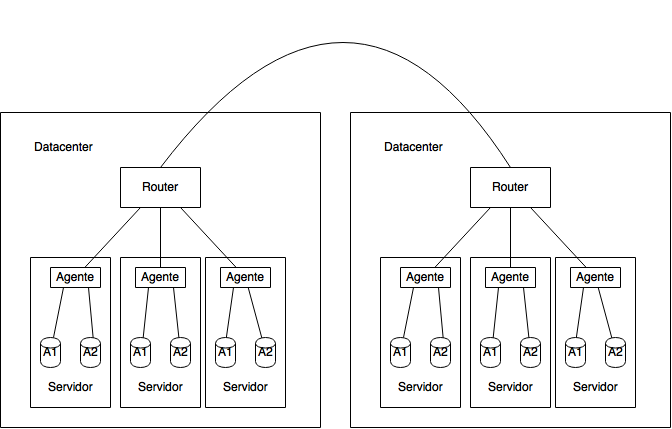
\includegraphics[width=15cm]{diagramas/datacenterx2.png}

\noindent
De esta forma podemos implementar replicaci'on de datos entre datacenters, y as'i si un datacenter se cae, no perdemos datos ni capacidad de proveer servicio a una regi'on.

\subsection{Repositorios}

Los repositorios forman parte de un esquema de almacenamiento de datos distribu'ido. Un repositorio distribu'ido en un datacenter contiene informaci'on sobre la regi'on en la que se encuentra el datacenter.

\begin{itemize}
	\item \textbf{Apuestas por partido.} Contiene las apuestas involucradas en cada partido en ejecuci'on.
	\item \textbf{Partidos pendientes y en ejecucion.} Contiene los partidos (tanto de desaf'io simulaci'on como fantas'ia) que est'an pendientes y en ejecuci'on.
	\item \textbf{Servidores simulando o transmitiendo partido.} Contiene los servidores que est'an simulando o transmitiendo cada partido.
	\item \textbf{Estad'isticas de jugador.} Contiene informaci'on estad'istica, como por ejemplo la cantidad de partidos ganados y perdidos, de cada jugador.
	\item \textbf{Informaci'on de eventos reales.} Contiene toda la informaci'on sobre eventos reales en los que se basan partidos fantas'ia.
	\item \textbf{Usuarios conectados a desaf'io.} Contiene ID e IP de los usuarios actualmente conectados a la sala de un desaf'io.
	\item \textbf{Regiones habilitadas para jugar.} Contiene las regiones a las que se les puede prestar servicio.
	\item \textbf{Regiones habilitadas para transmisi'on de partidos fantas'ia.} Contiene las regiones a las que se les puede transmitir un partido real desde 'esta regi'on.
	\item \textbf{Datos de jugador.} Contiene los datos de un jugador de la regi'on.
	\item \textbf{Estado de partido en ejecuci'on.} Contiene los datos de estado, por ejemplo puntaje de cada equipo, de los partidos que se est'an ejecutando en este momento.
	\item \textbf{Fixtures de desaf'ios.} Contiene los fixtures actualizados de los desaf'ios que a'un no acabaron. En particular, contiene los fixtures de los desaf'ios que a'un no han empezado.
	\item \textbf{Puntaje por acciones.} Contiene informaci'on sobre los par'ametros que se utilizan para puntuar las acciones que ocurren en un partido fantas'ia.
	\item \textbf{Premios por desaf'io.} Contiene los premios (monetarios y no monetarios) que se otorgan a los participantes desaf'ios que a'un no han acabado.
	\item \textbf{M'etodos de pago.} Contiene la informaci'on sobre los servicios de pago que se aceptan en 'esta regi'on.
	\item \textbf{Informaci'on de redes sociales.} Contiene la informaci'on m'as reciente descargada de redes sociales.
	\item \textbf{Publicidades.} Contiene las publicidades m'as recientes recibidas desde los proveedores de publicidad.
\end{itemize}

\subsubsection{Atributos de Calidad vs Arquitectura}
A continuacion listamos todos los atributos de calidad detallados en la seccion anterior y explicamos como hicimos para resolverlo en el diagrama de componentes y conectores.

\begin{itemize}
\item Atributo: El sistema debe evitar que los servidores superen su l'imite de clientes y se caigan.
\item Justificaci'on: Los componentes \textit{router} que reciben las peticiones de un cliente mantienen contadores acerca de la carga de los servidores. Cuando detectan una posible sobrecarga consultan la cantidad de usuarios conectados a los servidores de una regi'on. Lo hacen consultando el repositorio \textit{usuarios conectados a desaf'io}. Si hay sobrecarga, no se responde a las peticiones.

\item Atributo: Desea que haya un esfuerzo por respetar a los países en los que su legislación no permite que directamente se ingrese al sitio.
\item Justificacion: Los \textit{router} que reciban peticiones provenientes de regiones no habilitadas, no ser'an resueltas. Las regiones no habilitadas se consultan en el repositorio \textit{regiones habilitadas para jugar}.

\item Atributo: Se requiere que sea fácil desactivar una cuenta por un tiempo, para ayudar a los adictos en recuperación.
\item Justificacion: Se incluye un m'odulo para desactivar una cuenta, en el programa cliente.

\item Atributo: El simulador debe poder extenderse para soportar reglamentaciones nuevas ya que se espera poder incluir pa'ises adicionales.
\item Justificacion: La modificabilidad el simulador corre por cuenta de los desarolladores del mismo. En el caso del modo fantas'ia, cuya operatoria depende de nuestros desarrolladores, se incluye un repositorio con datos de configuraci'on para los partidos de dicho modo.

\item Atributo: El sistema debe correr en la mayor cantidad de plataformas posible. El sistema debe poder extenderse f'acilmente para incluir nuevas plataformas.
\item Justificacion: La arquitectura del sistema no asume requerimientos de hardware o software (salvo algunos muy b'asicos) sobre el cliente. Para poder soportar todo el abanico de dispositivos, desde aquellos con recursos de hardware y software limitados como aquellos de altas prestaciones, se incluyen dos motores gr'aficos, uno 3D (de altos requerimientos) y otro 2D (de bajos requerimientos). La decisi'on sobre cu'al utilizar se toma en base a los recursos disponibles al momento de la recepci'on de los resultados de la simulaci'on.

\item Atributo: 
\item Justificacion:

\item Atributo: 
\item Justificacion:

\item Atributo: 
\item Justificacion:
\end{itemize}


\end{document}
